\documentclass[12pt,a4paper]{article}

\usepackage[UTF8]{ctex}
\usepackage[scale=0.8]{geometry}
\usepackage{amsmath,amsfonts,amssymb,mathrsfs}
%\usepackage{txfonts,pxfonts,pifont,fontspec,bm}
\usepackage{abstract,appendix,diagbox,natbib,fancyhdr}
\usepackage{makeidx,hyperref}
\usepackage{graphicx,epsfig,subfig}
\usepackage{xcolor}

%\setlength{\lineskip}{\baselineskip}
\setlength{\parskip}{0.5\baselineskip}

\title{Anderson局部化实验报告8}
\author{sis-flag}
\date{\today}

\begin{document}
\maketitle

\section*{特征值的理论计算}

特征值问题
\begin{align*}
- u''(x) + V(x) u(x) = \lambda u(x) \qquad 0 < x < 1
\end{align*}
周期边界条件,$V(x)$是分片常数,取值为$0$或者$K$。

在$V(x)=0$处,方程变为
\begin{align*}
- u''(x) = \lambda u(x)
\end{align*}
取$\alpha = \sqrt{\lambda}$,它的通解为
\begin{align*}
u(x) = A \sin(\alpha x) + B \cos(\alpha x) \qquad u'(x) = A \alpha \cos(\alpha x) - B \alpha \sin(\alpha x)
\end{align*}
其中$A,B$是待定系数。

对于较小的几个特征值,满足$\lambda < K$。在$V(x)=K$处,方程变为
\begin{align*}
u''(x) = (K - \lambda) u(x)
\end{align*}
取$\beta = \sqrt{K - \lambda}$,它的通解为
\begin{align*}
u(x) = A \exp(\beta x) + B \exp(-\beta x) \qquad u'(x) = A \beta \exp(\beta x) - B \beta \exp(-\beta x)
\end{align*}

周期边界下,不妨设$V(0)=0, V(1)=K$。在不同的区域上,对应不同的待定系数。如图\ref{f0}。
\begin{figure}[h]
\centering
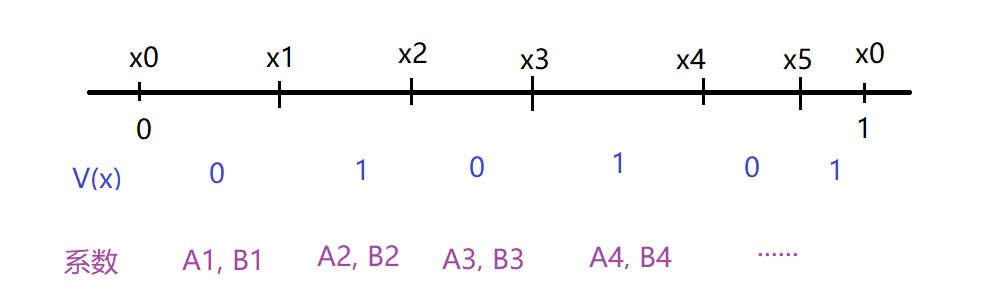
\includegraphics[width=0.7\linewidth]{0}
\caption{区域示意图}
\label{f0}
\end{figure}

我们要求特征函数的函数值连续,一阶导数也连续,加上周期边界条件,就得到了一系列方程约束
\begin{align*}
A_1 \sin(\alpha x_1) + B_1 \cos(\alpha x_1) & = A_2 \exp(\beta x_1) + B_2 \exp(-\beta x_1) \\
A_1 \alpha \cos(\alpha x_1) - B_1 \alpha \sin(\alpha x_1) & = A_2 \beta \exp(\beta x_1) - B_2 \beta \exp(-\beta x_1) \\
& \cdots
\end{align*}

记
\begin{align*}
G_i = \left[\begin{array}{cc}
\sin(\alpha x_i) & \cos(\alpha x_i) \\
\alpha \cos(\alpha x_i) & - \alpha \sin(\alpha x_i) \\
\end{array}\right]
\qquad
E_i = \left[\begin{array}{cc}
\exp(\beta x_i) & \exp(-\beta x_i) \\
\beta \exp(\beta x_i) & - \beta \exp(-\beta x_i) \\
\end{array}\right]
\end{align*}
可以得到
\begin{align*}
G_1 [A_1, B_1]^T & = E_1 [A_2, B_2]^T \\
E_2 [A_2, B_2]^T & = G_2 [A_3, B_3]^T \\
& \cdots \\
E_N [A_N, B_N]^T & = G_0 [A_1, B_1]^T
\end{align*}

如果$\lambda$是方程的特征值,就等价于下面这个方程有非零解
\begin{align*}
G_0^{-1} E_{N} E_{N-1}^{-1} G_{N-1} \cdots G_2^{-1} E_2 E_1^{-1} G_1 [A_1, B_1]^T = [A_1, B_1]^T
\end{align*}
就等价于系数矩阵行列式为零
\begin{align*}
D(\lambda) = \det(G_0^{-1} E_N E_{N-1}^{-1} G_{N-1} \cdots G_2^{-1} E_2 E_1^{-1} G_1 - I) = 0
\end{align*}

虽然这里面都是二阶的矩阵,但是在分段很多的时候,$D(\lambda)$的表达式会变得特别复杂。但是可以肯定的是,它是一个定义在$[0,K]$上的光滑函数。

如图\ref{f1}左边。图中蓝色的线是$D(\lambda)$的图像,黄色的线是$y=0$,黑色的点是用谱元法计算得到的特征值。(参数$K=1100$,$N=(7,20,5,1,5)$)
\begin{figure}[h]
\centering
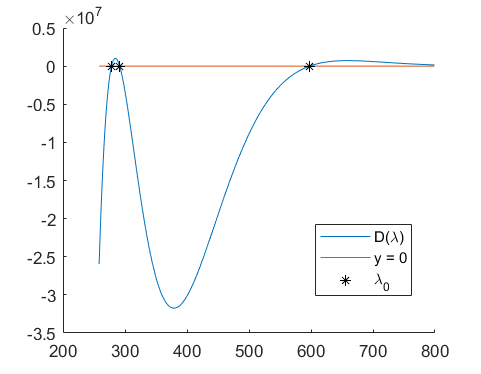
\includegraphics[width=0.4\linewidth]{1}
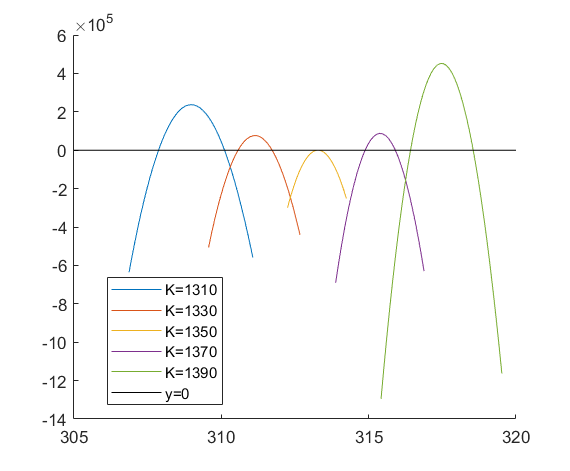
\includegraphics[width=0.4\linewidth]{2}
\caption{函数图像}
\label{f1}
\end{figure}

图\ref{f1}右边画出了不同$K$下的$D(\lambda)$图像。根据之前的分析,相变发生的时候,是特征值出现重根的时候,也就是函数$D(\lambda)$的零点是二重零点的时候。之前通过模拟,我们得到$N=(7,20,5,1,5)$情况下,相变点是$K=1351.22$。这和图中的结果也相符。

这里给出了一种不用模拟系统就能求解得到相变点的方法。

\section*{子区域特征值计算}

之前我们提到,localize到左边的特征函数对应一个特征值,localize到右边的对应一个特征值。它们随K增加而增长的变化速率不一样。由于我们关心“最小”特征值对应的特征函数,当一个特征值和另一个相等的时候,“最小”的特征值就从一个变成了另一个,从而发生了相变。下面我们更加深入地研究一下这个问题。

在计算其中一个子区域对应的特征值时,我们把另一个子区域内的$V(x)$取值改成0,就得到了两个子区域对应的势函数$V_1(x), V_2(x)$,示意图如图\ref{f5}图中深蓝色是取值为K的,浅蓝色是取值为0的区域。
\begin{figure}[h]
\centering
\subfloat[V1]{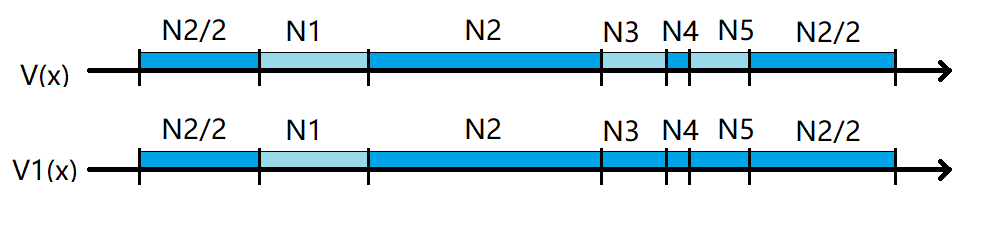
\includegraphics[width=0.49\linewidth]{51}}
\subfloat[V2]{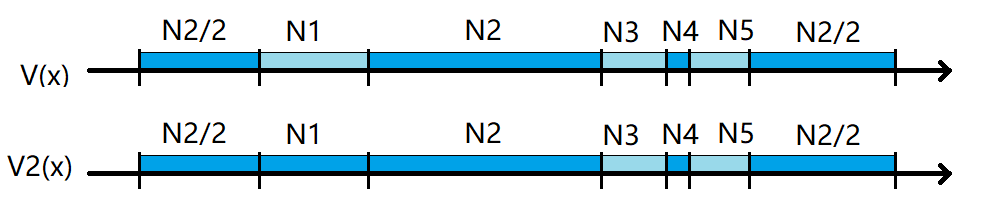
\includegraphics[width=0.49\linewidth]{52}}
\caption{势函数示意图}
\label{f5}
\end{figure}

计算两个子区域分别对应的特征值,得到结果如图\ref{f6}。在$V(x)$下的最小和第二小的特征函数和子区域上的几乎重合。参数$N=(7,20,5,1,5)$,第一张图里$K=1000$。计算得到的特征值为
$$ \lambda_1(V) = 263.3242; \ \lambda_2(V) = 281.1789; \ \lambda_1(V_1) = 263.3247; \ \lambda_1(V_2) = 281.1808; $$
图\ref{f6}(b)中画出了不同K下的原问题特征值和子区域问题特征值。
\begin{figure}[h]
\centering
\subfloat[特征函数]{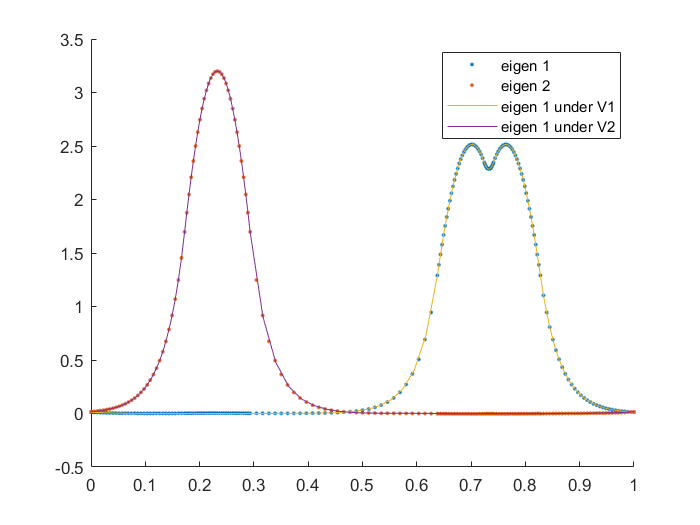
\includegraphics[width=0.4\linewidth]{61}}
\subfloat[特征值]{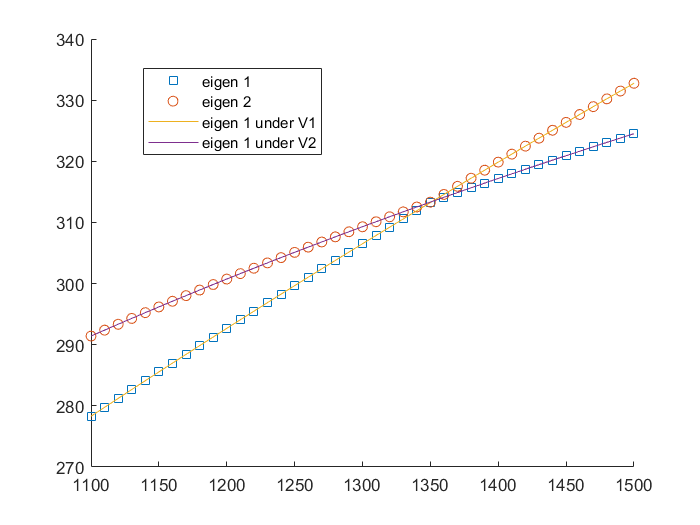
\includegraphics[width=0.4\linewidth]{62}}
\caption{模拟结果}
\label{f6}
\end{figure}

这里我们验证了总的特征值可以用两个区域对应的子特征值近似,下面我们试图从理论上求出子区域上的特征值。(这里考虑$N_3=N_5$的情况)

如图\ref{f5}。由于是周期边界条件,我们可以把一段0移动到正中间,而不改变特征值的数值。同时,又根据特征函数的对称性,把整个区间上的周期边界条件问题等价成半个区间上的Neumann边界条件问题。经过这些等价,我们终于可以计算出每个区间上特征值的理论表达式了。

\subsection*{$N_1$子区域特征值}

第一段子区域上,可以看成是在$[0, 1/2]$上,Neumann边界条件,在$[0, x_0]$上$V(x)$取值为$0$,其他部分取值为$K$的情况。其中$x_0 = L_1/2$。

在$[0, x_0]$上,通解为
\begin{align*}
u(x) = A \sin(\alpha x) + B \cos(\alpha x) \qquad u'(x) = A \alpha \cos(\alpha x) - B \alpha \sin(\alpha x)
\end{align*}
在$[x_0, 1/2]$上,通解为
\begin{align*}
u(x) = C \exp(\beta x) + D \exp(-\beta x) \qquad u'(x) = C \beta \exp(\beta x) - D \beta \exp(-\beta x)
\end{align*}

边界条件和连续性条件表示为
\begin{align*}
u'(0) & = A \alpha = 0 \\
u'(1/2) & = C \beta \exp(\beta/2) - D \beta \exp(-\beta/2) = 0 \\
u(x_0) & = A \sin(\alpha x_0) + B \cos(\alpha x_0) = C \exp(\beta x_0) + D \exp(-\beta x_0) \\
u'(x_0) & = A \alpha \cos(\alpha x_0) - B \alpha \sin(\alpha x_0) = C \beta \exp(\beta x_0) - D \beta \exp(-\beta x_0)
\end{align*}
系数矩阵为
\begin{align*}
\left[\begin{array}{cccc} \alpha & 0 & 0 & 0\\ 0 & 0 & \beta \mathrm{e}^{\frac{\beta}{2}} & - \beta \mathrm{e}^{-\frac{\beta}{2}}\\ \sin\!\left(\alpha x_0\right) & \cos\!\left(\alpha x_0\right) & - \mathrm{e}^{\beta x_0} & - \mathrm{e}^{- \beta x_0}\\ \alpha \cos\!\left(\alpha x_0\right) & - \alpha \sin\!\left(\alpha x_0\right) & - \beta \mathrm{e}^{\beta x_0} & \beta \mathrm{e}^{- \beta x_0} \end{array}\right]
\left[\begin{array}{c} A \\ B \\ C \\ D \end{array}\right]
=
\left[\begin{array}{c} 0 \\ 0 \\ 0 \\ 0 \end{array}\right]
\end{align*}

方程有非零解,就是系数矩阵行列式为0
\begin{align*}
\alpha \mathrm{e}^{2 \beta x_0} \sin\!\left(\alpha x_0\right) - \beta \mathrm{e}^{\beta} \cos\!\left(\alpha x_0\right) + \alpha \mathrm{e}^{\beta} \sin\!\left(\alpha x_0\right) + \beta \mathrm{e}^{2 \beta x_0} \cos\!\left(\alpha x_0\right) = 0
\end{align*}
化简得到
\begin{align*}
D_1(K, \lambda) = \alpha \tan(\alpha x_0) - \beta \tanh(\beta (\frac12 - x_0)) = 0
\end{align*}

\subsection*{$N_3$子区域特征值}

第二段子区域上,可以看成是在$[0, 1/2]$上,Neumann边界条件,在$[0, x_1]$和$[x_2, 1/2]$上$V(x)$取值为$K$,其他部分取值为$0$的情况。其中$x_1 = N_4/2, x_2 = N_4/2 + N_3$

在$[0, x_1]$上,通解为
\begin{align*}
u(x) = A \exp(\beta x) + B \exp(-\beta x) \qquad u'(x) = A \beta \exp(\beta x) - B \beta \exp(-\beta x)
\end{align*}
在$[x_1, x_2]$上,通解为
\begin{align*}
u(x) = C \sin(\alpha x) + D \cos(\alpha x) \qquad u'(x) = C \alpha \cos(\alpha x) - D \alpha \sin(\alpha x)
\end{align*}
在$[x_2, 1/2]$上,通解为
\begin{align*}
u(x) = E \exp(\beta x) + F \exp(-\beta x) \qquad u'(x) = E \beta \exp(\beta x) - F \beta \exp(-\beta x)
\end{align*}

边界条件和连续性条件表示为
\begin{align*}
u'(0) & = A \beta - B \beta = 0 \\
u(x_1) & = A \exp(\beta x_1) + B \exp(-\beta x_1) = C \sin(\alpha x_1) + D \cos(\alpha x_1) \\
u'(x_1) & = A \beta \exp(\beta x_1) - B \beta \exp(-\beta x_1) = C \alpha \cos(\alpha x_1) - D \alpha \sin(\alpha x_1) \\
u(x_2) & = C \sin(\alpha x_2) + D \cos(\alpha x_2) = E \exp(\beta x_2) + F \exp(-\beta x_2) \\
u'(x_2) & = C \alpha \cos(\alpha x_2) - D \alpha \sin(\alpha x_2) = E \beta \exp(\beta x_2) - F \beta \exp(-\beta x_2) \\
u'(1/2) & = E \beta \exp(\beta/2) - F \beta \exp(-\beta/2) = 0
\end{align*}

系数矩阵为
\begin{align*}
\left[\begin{array}{cccccc} 1 & -1 & 0 & 0 & 0 & 0\\ \mathrm{e}^{\beta x_1} & \mathrm{e}^{- \beta x_1} & - \sin\!\left(\alpha x_1\right) & - \cos\!\left(\alpha x_1\right) & 0 & 0\\ \beta \mathrm{e}^{\beta x_1} & - \beta \mathrm{e}^{- \beta x_1} & - \alpha \cos\!\left(\alpha x_1\right) & \alpha \sin\!\left(\alpha x_1\right) & 0 & 0\\ 0 & 0 & \sin\!\left(\alpha x_2\right) & \cos\!\left(\alpha x_2\right) & - \mathrm{e}^{\beta x_2} & - \mathrm{e}^{- \beta x_2}\\ 0 & 0 & \alpha \cos\!\left(\alpha x_2\right) & - \alpha \sin\!\left(\alpha x_2\right) & - \beta \mathrm{e}^{\beta x_2} & \beta \mathrm{e}^{- \beta x_2}\\ 0 & 0 & 0 & 0 & \mathrm{e}^{\frac{\beta}{2}} & - \mathrm{e}^{-\frac{\beta}{2}} \end{array}\right]
\end{align*}

方程有非零解,就是系数矩阵行列式为0
\begin{align*}
& \alpha^2 \mathrm{e}^{2 \beta (x_{1} + x_{2})}  + \alpha^2 \mathrm{e}^{2 \beta (x_{1} + x_{3})} \\
+ & \beta^2 \mathrm{e}^{2 \beta (x_{1} + x_{2})} - \beta^2 \mathrm{e}^{2 \beta (x_{1} + x_{3})} \\
+ & \alpha^2 \mathrm{e}^{2 \beta x_{2}}  + \alpha^2 \mathrm{e}^{2 \beta x_{3}} \\
- & \beta^2 \mathrm{e}^{2 \beta x_{2}} + \beta^2 \mathrm{e}^{2 \beta x_{3}} \\
+ & 2 \alpha \beta \mathrm{e}^{2 \beta (x_{1} + x_{3})} \cot(\alpha (x_{1} - x_{2})) - 2 \alpha \beta \mathrm{e}^{2 \beta x_{2}} \cot(\alpha (x_{1} - x_{2})) = 0
\end{align*}

化简得到
\begin{align*}
D_2(K, \lambda) = & (\alpha^2 - \beta^2)(\mathrm{e}^{2 \beta x_2} + \mathrm{e}^{2 \beta (x_1+x_3)}) / (\mathrm{e}^{2 \beta (x_1+x_3)} - \mathrm{e}^{2 \beta x_2}) \\
+ & (\alpha^2 + \beta^2)(\mathrm{e}^{2 \beta x_3} + \mathrm{e}^{2 \beta (x_1+x_2)}) / (\mathrm{e}^{2 \beta (x_1+x_3)} - \mathrm{e}^{2 \beta x_2}) \\
+ & 2 \alpha \beta \cot(\alpha (x_1 - x_2))= 0
\end{align*}
其中$x_3 = \frac12$

发生相变的时候,两个方程的零点相同,所以我们就得到了相变点满足的方程组为
\begin{align*}
D_1(K, \lambda) = 0 \\
D_2(K, \lambda) = 0
\end{align*}
方程组的解$K$就是相变点,解$\lambda$就是相变时的特征值。

图\ref{fD}中展示了通过求解方程组得到的和模拟物理过程得到的结果对比。图中横轴是相变点和相变处特征值的预测值,纵轴是模拟得到的值,红色线是$x=y$直线。可以看出,在相变点和特征值不是特别大的时候,预测的结果都很好。
\begin{figure}[h]
\centering
\subfloat[相变点]{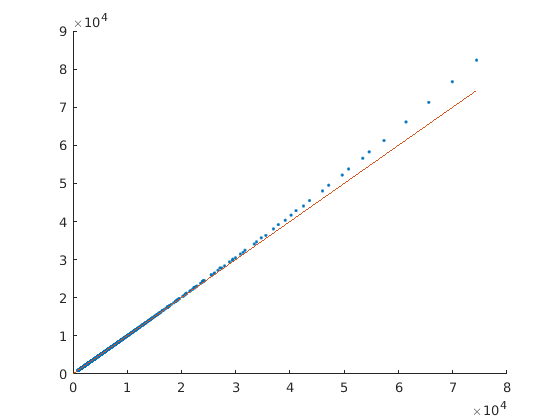
\includegraphics[width=0.4\linewidth]{DfK}}
\subfloat[特征值]{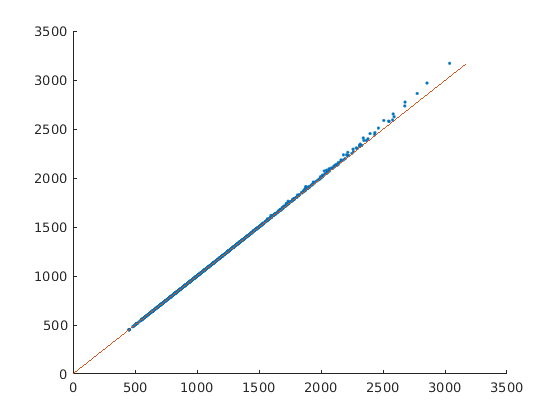
\includegraphics[width=0.4\linewidth]{Dfl}}
\caption{模拟结果和预测结果}
\label{fD}
\end{figure}

\section*{landscape和特征函数之间的关系}

我们猜测,landscape最高的峰,对应最小特征函数的峰。下面我们分别随机生成势函数,找到landscape前几个峰值的位置$x^{(l)}$,和前几个特征值峰的位置$x^{(e)}$。计算它们之间的差异。

图中横轴是特征值序号,纵轴展示了landscape的峰和特征函数的峰值位置之间的差异。图中参数为$K=1e6, h=10$,势函数分片数$N=50$,共采样$1000$次。图\ref{ml1}是Bernoulli分布($p=0.5$)的结果,图\ref{ml2}中是均匀分布的结果。
\begin{figure}[h]
\centering
\subfloat[差异箱线图$x^{(l)} - x^{(e)}$]{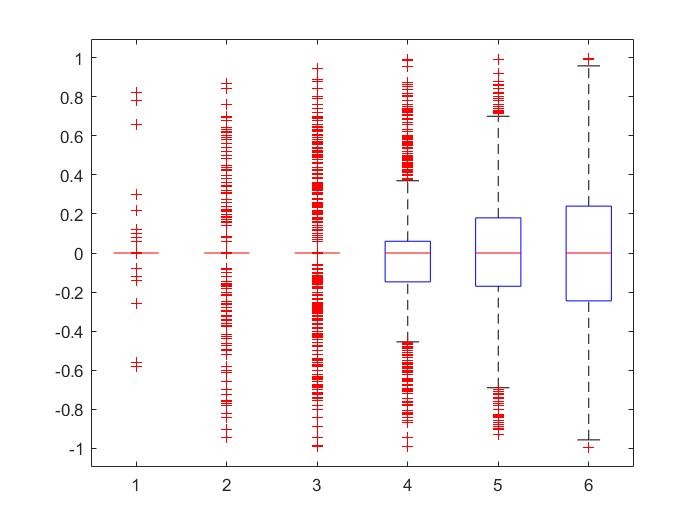
\includegraphics[width=0.3\linewidth]{bx_p5}}
\subfloat[均方误差$\sum |x^{(l)} - x^{(e)}|^2$]{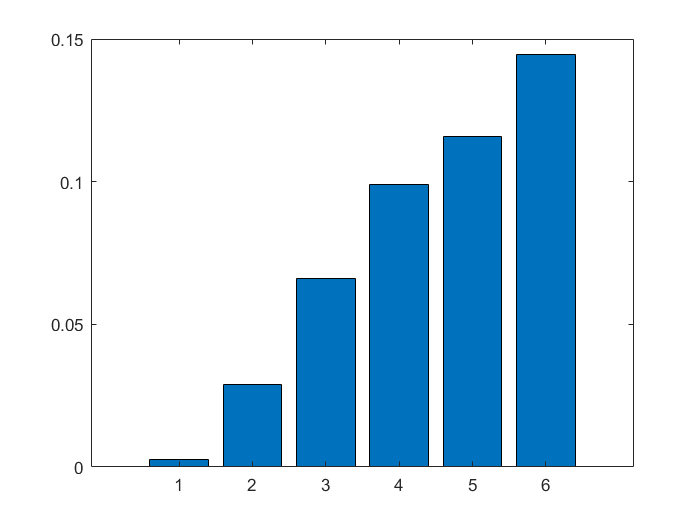
\includegraphics[width=0.3\linewidth]{mse_p5}}
\caption{landscape的峰和特征函数的峰值位置差异($P=0.5$)}
\label{ml1}
\end{figure}
\begin{figure}[h]
\centering
\subfloat[差异箱线图$x^{(l)} - x^{(e)}$]{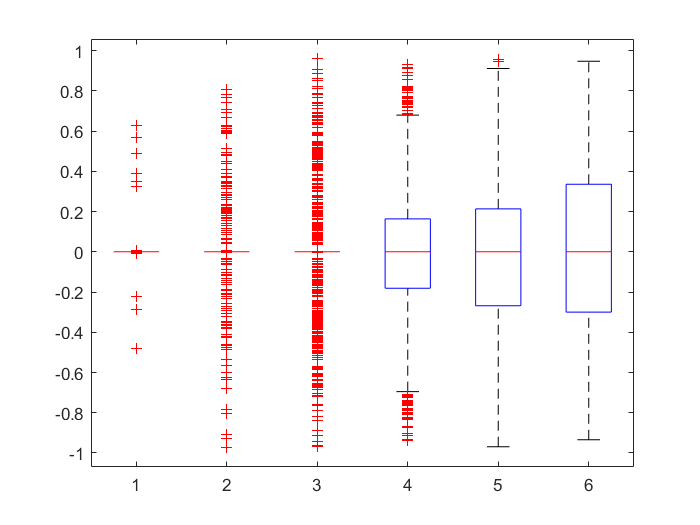
\includegraphics[width=0.3\linewidth]{bx_p0}}
\subfloat[均方误差$\sum |x^{(l)} - x^{(e)}|^2$]{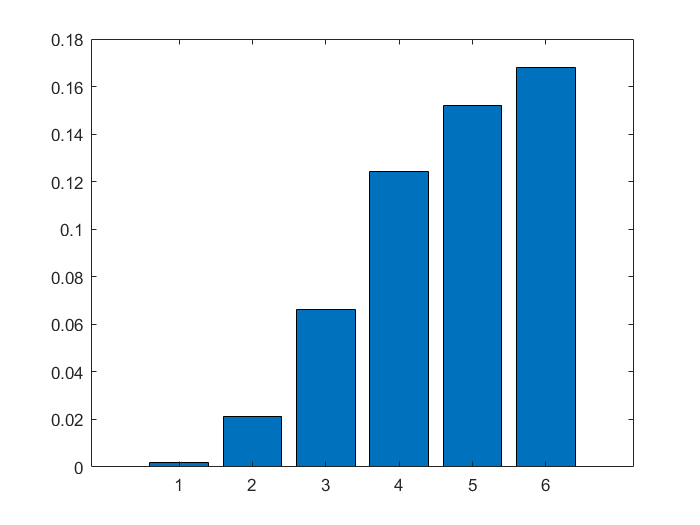
\includegraphics[width=0.3\linewidth]{mse_p0}}
\caption{landscape的峰和特征函数的峰值位置差异(均匀分布)}
\label{ml2}
\end{figure}

我们同样统计了二维情况下的结果,由于计算量限制,我们计算的是$10\times10$的分片,采样$200$次。结果如图\ref{ml3}。二维情况下无法比较大小,只能计算均方误差了。
\begin{figure}[h]
\centering
\subfloat[Bernoulli分布($p=0.5$)]{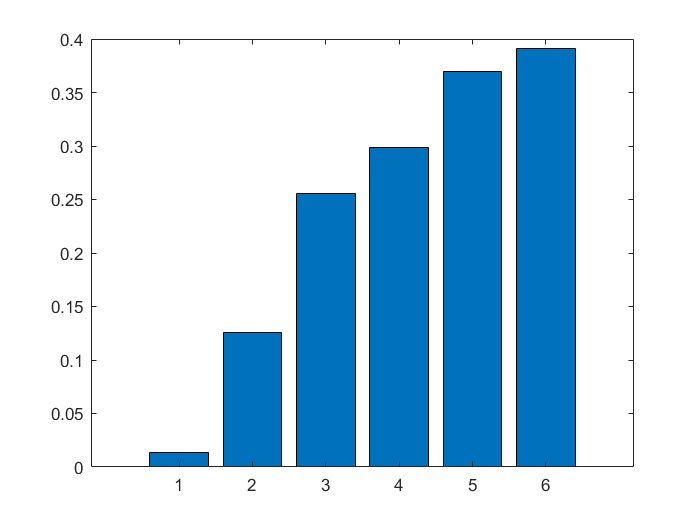
\includegraphics[width=0.3\linewidth]{mse_p5_2d}}
\subfloat[均匀分布]{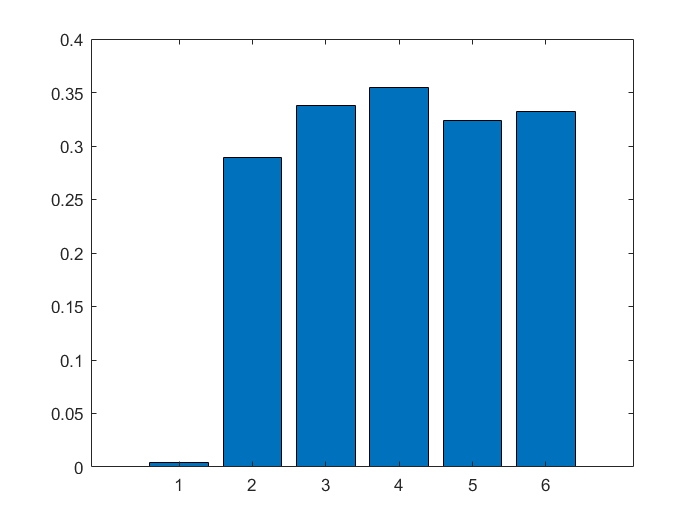
\includegraphics[width=0.3\linewidth]{mse_p0_2d}}
\caption{landscape的峰和特征函数的峰值位置均方误差(二维)}
\label{ml3}
\end{figure}

从图中可以看出,编号稍大的特征函数可能误差较大,但是对于最小特征值对应的特征函数,这样的猜想还是很可靠的。

\section*{两段一样长的概率}

这里我们关注一维的情况。如图\ref{f3},有的时候,最小特征值对应的特征函数有两个峰。根据之前的分析,这种情况会出现在最长的两段连续的0相等的时候。图中紫色和黄色的线是最小和第二小的特征函数,蓝色的部分代表$V(x)$在此处取值为$K$,否则取值为$0$。
\begin{figure}[h]
\centering
\subfloat[Dirichlet边界]{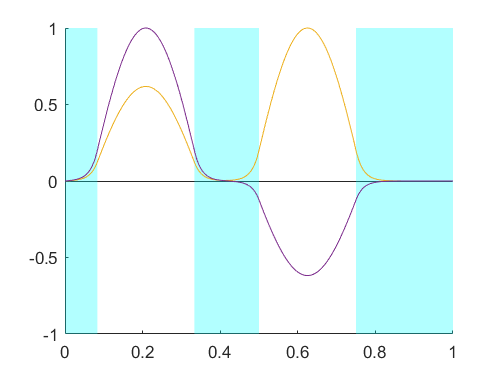
\includegraphics[width=0.24\linewidth]{31}}
\subfloat[Dirichlet边界]{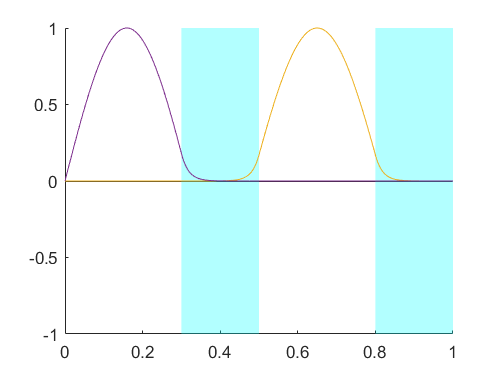
\includegraphics[width=0.24\linewidth]{32}}
\subfloat[Neumann边界]{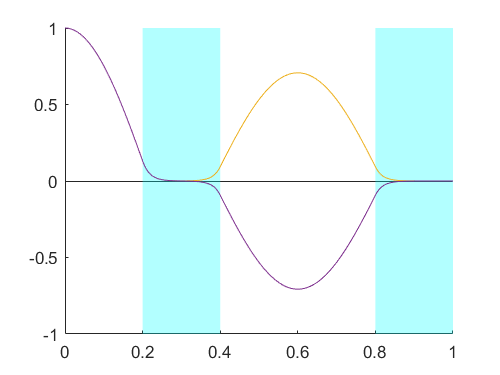
\includegraphics[width=0.24\linewidth]{33}}
\subfloat[Neumann边界]{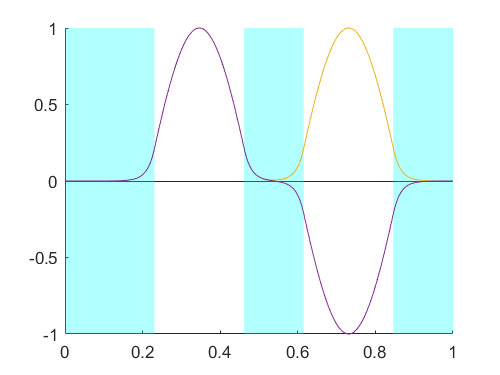
\includegraphics[width=0.24\linewidth]{34}}
\caption{特征函数图像}
\label{f3}
\end{figure}
需要注意的是,在Dirichlet边界下,有可能出现图(b)中的情况,如果最长的一段位于边界,就不会出现双峰的情况。另一方面,在Neumann边界下,边界附近的长度要按二倍计算。

后面又模拟了一些结果,发现\textbf{特征值的双峰并不是完全和“两段一样长”这个事件等价,具体原因不明},也有可能是模拟误差的问题。如图\ref{ff},图中紫色和黄色的线是最小和第二小的特征函数。
\begin{figure}[h]
\centering
\subfloat[Dirichlet边界]{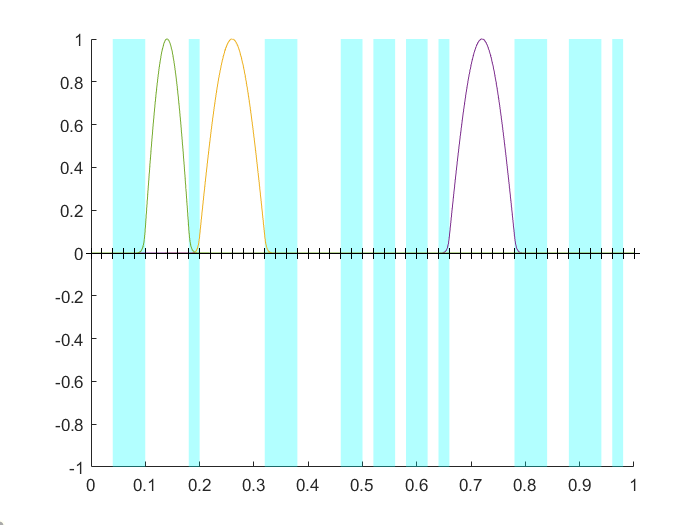
\includegraphics[width=0.4\linewidth]{3f}}
\caption{特征函数图像}
\label{ff}
\end{figure}

图\ref{f4}中,蓝色线是对“两段一样长”概率的预测值,紫色线是模拟过程中“两段一样长”出现的频率,红色的线是模拟过程中最小特征函数出现多个峰的频率。
\begin{figure}[h]
\centering
\subfloat[Dirichlet边界]{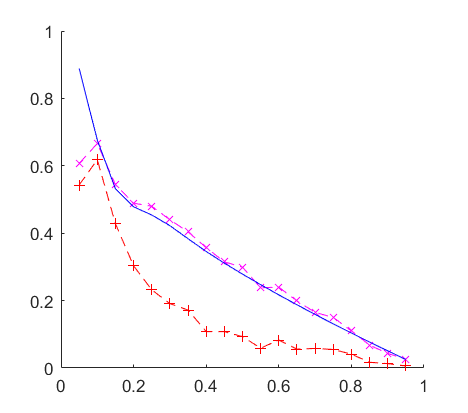
\includegraphics[width=0.4\linewidth]{4f}}
\caption{概率和频率}
\label{f4}
\end{figure}

%根据之前的结果,设$M = N p q$,在平均的意义下,我们可以近似地认为长度为$X_1, Y_1, \cdots, X_M, Y_M$的取值相同的段组成。
%
%这些随机变量$X$近似服从相互独立的几何分布
%$$ \mathbb{P}(X = n) = p^{n-1} q $$
%均值$E(X) = 1/q$。而且
%$$ \mathbb{P}(X < n) = 1 - p^{n-1} $$

%\subsection*{Dirichlet边界条件}
%
%情况很复杂
%
%\paragraph*{情况1}
%两端取值都为$0$,这种情况出现的概率为$p^2$。
%
%我们所求的概率为
%\begin{align*}
%  & \mathbb{P}(\max\{X_2, X_3, \cdots, X_{M-1}\} \leq 2 \max\{X_1, X_M\}) \\
%= & \sum_{m,n=1}^{\infty} \mathbb{P}(\max\{X_2, X_3, \cdots, X_{M-1}\} < 2 \max\{m,  n\}) \mathbb{P}(X_1 = m) \mathbb{P}(X_M = n) \\
%= & \sum_{m,n=1}^{\infty} [\mathbb{P}(X_i < 2 \max\{m,n\}) ]^{M-2} \mathbb{P}(X_1 = m) \mathbb{P}(X_M = n)\\
%= & \sum_{m,n=1}^{\infty} (1 - p^{2 \max\{m,n\}-1})^{M-2} p^{m-1} q p^{n-1} q\\
%= & \sum_{k=1}^{\infty} p^{k-2} q^2 \sum_{n=1}^{k-1} (1 - p^{2 \max\{k-n,n\}-1})^{M-2} 
%%\end{align*}

%\paragraph*{情况2}
%左边取值为$0$,右边取值为$1$,这种情况出现的概率为$pq$。
%
%我们所求的概率为
%\begin{align*}
%  & \mathbb{P}(\max\{X_2, X_3, \cdots, X_{M}\} < 2 X_1) \\
%= & \sum_{n=1}^{\infty} \mathbb{P}(\max\{X_2, X_3, \cdots, X_{M-1}\} < n) \mathbb{P}(X_1 = n) \\
%= & \sum_{n=1}^{\infty} [\mathbb{P}(X_i < 2 n]^{M-1} \mathbb{P}(X_1 = n)\\
%= & q \sum_{n=1}^{\infty} (1 - p^{2 n-1})^{M-2} p^{n-1}
%\end{align*}

\end{document}